% NeurIPS 2026 Preprint -- Work in Progress
% Last updated: April 2026
%
% Build with: make paper (from project root)
% See paper/WORKFLOW.md for AI agent instructions

\documentclass{article}

% NeurIPS 2026 style (preprint mode)
\usepackage[preprint]{neurips_2026}

% Recommended packages
\usepackage[utf8]{inputenc}
\usepackage[T1]{fontenc}
\usepackage{microtype}
\usepackage{graphicx}
\usepackage{subcaption}
\usepackage{booktabs}
\usepackage{hyperref}
\usepackage{url}
\usepackage{amsmath,amssymb,mathtools,amsthm}
\usepackage[capitalize,noabbrev]{cleveref}
\usepackage{algorithm}
\usepackage{algorithmic}
\usepackage{enumitem}

% Path to figures (relative to paper/ directory, set via TEXINPUTS)
\graphicspath{{../figures/}}

%%%%%%%%%%%%%%%%%%%%%%%%%%%%%%%%
% THEOREMS AND MACROS
%%%%%%%%%%%%%%%%%%%%%%%%%%%%%%%%

\theoremstyle{plain}
\newtheorem{theorem}{Theorem}[section]
\newtheorem{proposition}[theorem]{Proposition}
\newtheorem{lemma}[theorem]{Lemma}
\newtheorem{corollary}[theorem]{Corollary}
\theoremstyle{definition}
\newtheorem{definition}[theorem]{Definition}
\newtheorem{assumption}[theorem]{Assumption}
\newtheorem{axiom}[theorem]{Axiom}
\theoremstyle{remark}
\newtheorem{remark}[theorem]{Remark}

\newcommand{\R}{\mathbb{R}}
\newcommand{\E}{\mathbb{E}}
\newcommand{\Q}{\hat{Q}}
\DeclareMathOperator{\KL}{KL}
\DeclareMathOperator{\Var}{Var}
\DeclareMathOperator{\Cov}{Cov}

\title{MALA-Guided Mirror Descent:\\Inference-Time Q-Guidance for Diffusion Policy RL\\[0.5em]\normalsize\textit{Preprint -- Work in Progress}}

\author{%
  Philip Nielsen \\
  Harvard University\\
  \texttt{pnielsen@seas.harvard.edu} \\
}

\begin{document}

\maketitle

\begin{abstract}
We approach the problem of online reinforcement learning (RL) for continuous control tasks through the lens of pure optimization. Given a policy and tilting signal Q, we aim to identify the optimal target policy and update toward it as accurately as possible. 
To this end, motivated by a principle of self-consistency, we restrict to the $\alpha$-divergence mirror descent class of policy updates. 
We introduce MALA-guidance, a guidance procedure for diffusion models which admits arbitrary scaling of compute to improve the accuracy with which samples are drawn from the desired target distribution. We show that, with this method, diffusion policies can be tilted accurately enough to achieve stable online RL simply by continuously distilling guided actions back into the base policy through standard supervised learning. 
To further identify the optimal policy target, we adaptively tune the parameters of the target update by modeling the induced state distribution shift and resulting shift in value estimates. This enables the method to continuously adjust its update rule in response to the training dynamics and environment, eliminating the need to tune hyperparameters for each task.
Our approach significantly improves sample efficiency over prior model-free non-distributional RL methods in continuous control tasks.
\end{abstract}



\section{Introduction}
\label{sec:intro}

one sentence context
problem

Diffusion models \citep{ho2020denoising,song2021sde} have emerged as a powerful policy class for reinforcement learning (RL), with a growing body of work applying them in offline RL \citep{janner2022diffuser,wang2023diffusion,hansen2023idql}, online RL \citep{ma2025soft,yang2023dipo}, and inference-time policy extraction \citep{park2025fql,espinosa2025sorl,espinosa2025evor}.
Unlike standard Gaussian policies, which generate actions in a single forward pass, diffusion policies are a more expressive policy class that produces actions through an iterative denoising process.
This expressiveness matters for policy improvement: the mirror descent update $\pi_{\mathrm{new}}(a|s) \propto \pi_{\mathrm{old}}(a|s)\exp\{\eta Q(s,a)\}$ does not in general remain Gaussian even when $\pi_{\mathrm{old}}$ is, so less expressive policy classes must project back onto their parametric family, losing information. Diffusion policies can represent the tilted distribution directly.
Moreover, recent evidence suggests that the iterative structure of diffusion---not expressiveness per se---is the principal driver behind their strong empirical performance \citep{pan2024mip}, as it enables per-step refinement and the injection of external guidance signals.
This raises a fundamental question: \emph{given a learned value function $Q(s,a)$, how should we use it to improve a diffusion policy?}

\begin{figure}[t]
  \centering
  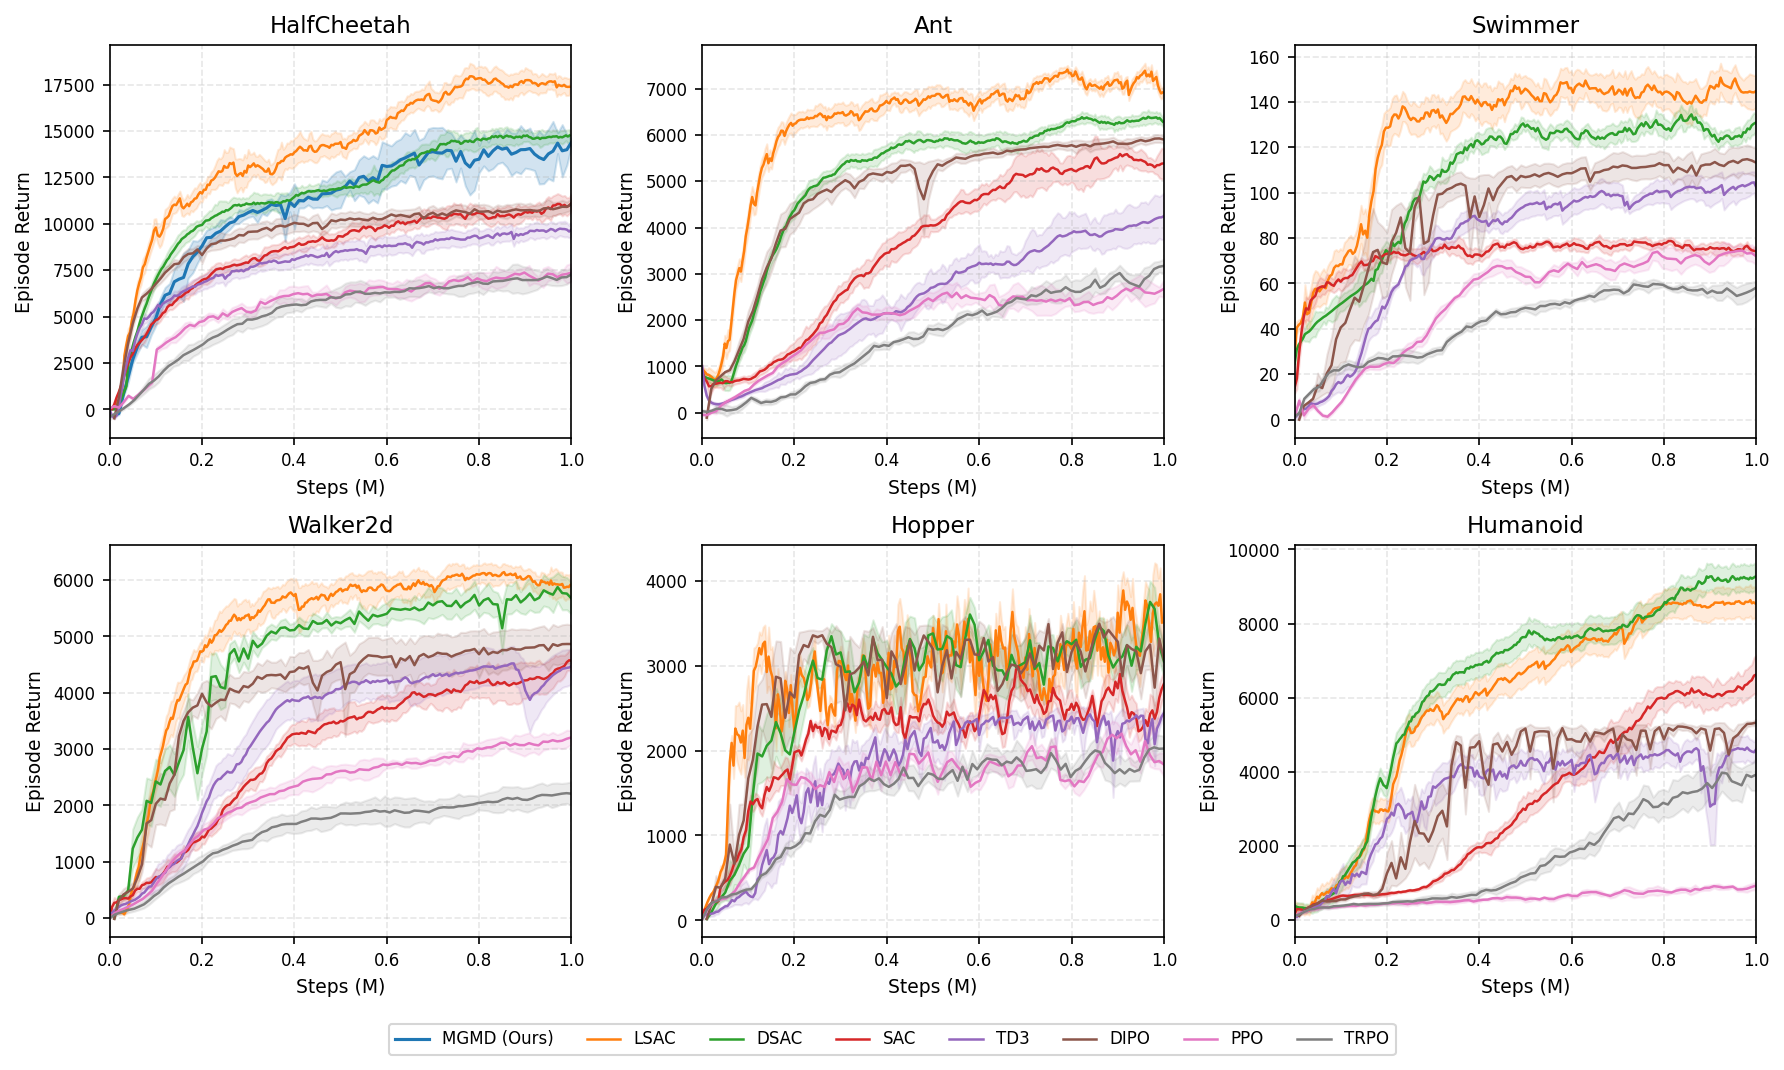
\includegraphics[width=\textwidth]{model_free_training_curves_all_envs.png}
  \caption{Training curves across 6 MuJoCo environments comparing MGMD against baselines from \citet{lsac2025} over 10 seeds. MGMD reports 1 seed for non-HalfCheetah for now. Shaded regions show 90\% CI via $t$-distribution.}
  \label{fig:training-curves}
  \vskip -0.1in
\end{figure}

\begin{table}[t]
  \caption{Final episode return on MuJoCo benchmarks (mean $\pm$ 90\% CI). Values are the final evaluation point of a $10^6$ step training run. Baselines from \citet{lsac2025} use 10 seeds; MGMD uses 10 seeds on HalfCheetah and 1 seed elsewhere ($^\dagger$). CI computed via $t$-distribution. Bold indicates best.}
  \label{tab:main-results}
  \vskip 0.1in
  \begin{center}
  \begin{small}
  \resizebox{\textwidth}{!}{%
  \begin{tabular}{lccccccccc}
    \toprule
    Environment & MGMD (Ours) & DPMD & EXPO & RedQ & DIPO & SAC & TD3 & PPO & TRPO \\
    \midrule
    HalfCheetah & $\mathbf{15385{\scriptstyle\pm279}}$ & $\text{---}$ & $\text{---}$ & $10022{\scriptstyle\pm1298}$ & $11064{\scriptstyle\pm325}$ & $11114{\scriptstyle\pm494}$ & $9692{\scriptstyle\pm363}$ & $7371{\scriptstyle\pm496}$ & $7277{\scriptstyle\pm349}$ \\
    Ant & $5090^\dagger$ & $\text{---}$ & $\text{---}$ & $\mathbf{6091{\scriptstyle\pm129}}$ & $5900{\scriptstyle\pm77}$ & $5385{\scriptstyle\pm328}$ & $4247{\scriptstyle\pm500}$ & $2676{\scriptstyle\pm186}$ & $3171{\scriptstyle\pm143}$ \\
    Walker2d & $\mathbf{5328}^\dagger$ & $\text{---}$ & $\text{---}$ & $4598{\scriptstyle\pm318}$ & $4864{\scriptstyle\pm340}$ & $4568{\scriptstyle\pm214}$ & $4474{\scriptstyle\pm319}$ & $3208{\scriptstyle\pm120}$ & $2210{\scriptstyle\pm210}$ \\
    Hopper & $2081^\dagger$ & $\text{---}$ & $\text{---}$ & $\mathbf{3002{\scriptstyle\pm512}}$ & $3071{\scriptstyle\pm171}$ & $2784{\scriptstyle\pm154}$ & $2441{\scriptstyle\pm50}$ & $1835{\scriptstyle\pm137}$ & $2023{\scriptstyle\pm145}$ \\
    Humanoid & $3933^\dagger$ & $\text{---}$ & $\text{---}$ & $\mathbf{7213{\scriptstyle\pm621}}$ & $5330{\scriptstyle\pm87}$ & $6628{\scriptstyle\pm529}$ & $4620{\scriptstyle\pm313}$ & $938{\scriptstyle\pm105}$ & $3932{\scriptstyle\pm438}$ \\
    Swimmer & $\mathbf{121}^\dagger$ & $\text{---}$ & $\text{---}$ & $134{\scriptstyle\pm22}$ & $113{\scriptstyle\pm6}$ & $74{\scriptstyle\pm2}$ & $102{\scriptstyle\pm6}$ & $72{\scriptstyle\pm4}$ & $58{\scriptstyle\pm3}$ \\
    \bottomrule
  \end{tabular}%
  }
  \end{small}
  \end{center}
  \vskip -0.1in
\end{table}

This is an instance of the \emph{policy extraction} problem, which \citet{park2024bottleneck} identify as a critical bottleneck---often more impactful than value learning itself.
For standard Gaussian policies, reparameterized policy gradients provide a direct solution.
For diffusion policies, the iterative sampling process makes this non-trivial, and existing approaches fall into three categories:
\begin{enumerate}
  \item \textbf{Weighted behavioral cloning.} DPMD \citep{ma2025soft} reweights the denoising loss by $\exp\{\eta Q(s,a)\}$, implementing the mirror-descent update $\pi(a\mid s) \propto \pi_\mathrm{old}(a\mid s) \exp\{\eta Q(s,a)\}$ (see \cref{eq:md-tilt}) at training time. This is analogous to advantage-weighted regression (AWR), which \citet{park2024bottleneck} show does not fully leverage the learned value function: when $Q$-values vary substantially across a batch, the exponentiated weights become heavy-tailed, concentrating gradient signal on a few high-$Q$ transitions and effectively discarding information from the rest.
  \item \textbf{Backpropagation through time (BPTT).} One can directly backpropagate $\nabla_a Q$ through the iterative denoising process, but this is often unstable and computationally expensive \citep{park2025fql}.
  \item \textbf{Rejection sampling.} Methods such as best-of-$N$ selection \citep{ma2025soft,espinosa2025evor} sample multiple action candidates and select the highest-$Q$ one. This uses no gradient information and scales poorly with action dimensionality.
\end{enumerate}

\noindent Notably, none of these approaches directly use $\nabla_a Q$ in a stable manner. \citet{park2024bottleneck} show that gradient-based policy extraction (e.g., DDPG+BC, which optimizes $\nabla_a Q$ directly) consistently outperforms both weighted BC and rejection sampling. Yet applying gradient-based extraction to diffusion policies has remained difficult due to the iterative sampling process.

More broadly, any policy network with fixed weights is an amortized optimizer that suffers an \emph{amortization gap}---the inability to perfectly optimize $Q$ for each individual state \citep{marino2021iterative}. Inference-time iterative refinement can close this gap, and recent large-scale studies confirm that inference strategies can break through the performance ceilings of well-trained RL policies \citep{chalumeau2025breaking}.

\paragraph{Our approach: MALA-Guided Mirror Descent (MGMD).}
We propose a simple resolution: train the diffusion policy with stable, unweighted behavioral cloning, and perform all $Q$-based policy improvement at inference time using gradient-based MCMC.
Specifically, at each noise level of the reverse diffusion process, we apply Metropolis-Adjusted Langevin Algorithm (MALA) corrections that use $\nabla_a Q$ to steer samples toward high-value regions, with Metropolis--Hastings acceptance to ensure accurate sampling from the tilted distribution.
This approach combines the training stability of pure BC with the effectiveness of gradient-based policy extraction---analogous to DDPG+BC but implemented at inference time via MCMC rather than at training time via policy gradients.

MGMD cleanly separates training and inference:
\begin{enumerate}
  \item \textbf{Training:} Fit the diffusion policy by unweighted behavioral cloning on replay buffer actions. In the online setting, these are the guided actions from prior iterations, so the BC loss distills the inference-time improvement into the base network. Train a standard twin Q-network via TD learning.
  \item \textbf{Inference:} At each diffusion noise level, apply MALA corrections using $\nabla_a Q$ to sample from the $Q$-tilted distribution $\pi(a|s) \propto \pi_\mathrm{old}(a|s)\exp\{\eta Q(s,a)\}$.
\end{enumerate}
The key insight is that policy improvement is fundamentally two problems: \emph{determining which actions should have been taken} (hard---even for bounded $\eta$, the tilted distribution $\pi \propto \pi_{\mathrm{old}} \exp(\eta Q)$ can be arbitrarily complex depending on the $Q$-landscape, requiring iterative refinement to sample accurately) and \emph{fitting the generative model to those actions} (easy, a standard supervised learning objective).
MGMD decouples these cleanly: the MALA-corrected guidance with $\nabla_a Q$ targets the exact mirror descent tilt distribution in theory, handling the hard problem at inference time, while the BC loss handles the easy problem at training time.
Because the replay buffer stores guided (post-MALA) actions, the BC loss implicitly distills the inference-time policy improvement back into the base network, enabling iterative improvement---a loop structurally analogous to AlphaGo Zero \citep{silver2017mastering}, which uses MCTS to produce actions better than the policy network alone, then trains the network to match.
This separation provides several advantages: (i) the diffusion loss is simple and stable, with no effective-sample-size issues from importance weights; (ii) constant learning rates support continual learning without horizon-dependent schedules; (iii) $\nabla_a Q$ is used directly, fully leveraging the learned value function; (iv) inference-time compute can be scaled independently of training by adjusting the number of MALA steps or particles, following the emerging paradigm of test-time compute scaling that has proven effective in game-playing \citep{silver2017mastering} and language modeling \citep{snell2024scaling}; and (v) the guidance strength $\eta$ can be set adaptively via a principled rule derived from a second-order expansion of policy improvement that accounts for distribution shift (\cref{sec:adaptive-eta}).

Our key finding is that unweighted training plus MALA guidance achieves strong performance on MuJoCo benchmarks, demonstrating that gradient-based inference-time policy extraction is an effective alternative to training-time reweighting for diffusion policy RL.

\section{Related Work}
\label{sec:related}

We organize our discussion of related work around the key components of our approach: diffusion models and guidance mechanisms, diffusion policies for RL, and inference-time action selection.

\paragraph{Diffusion models and guidance.}
Denoising diffusion probabilistic models (DDPMs) \citep{ho2020denoising} and score-based SDE models \citep{song2021sde} learn to reverse a gradually noised forward process.
Classifier guidance \citep{dhariwal2021beatgans} and classifier-free guidance \citep{ho2022classifierfree} modify the sampling dynamics by adding gradients of external or internal classifiers.
Training-free guidance (TFG) frameworks \citep{ye2024tfg,bansal2023universal} generalize this idea to arbitrary objectives evaluated on Tweedie-style clean estimates and highlight the need for careful treatment of guidance strength and off-manifold drift.
Energy-based diffusion with MCMC corrections \citep{du2023reduce_reuse_recycle} shows how to combine energy terms with the base diffusion model while correcting the sampler via Metropolis--Hastings steps.
These techniques have been applied primarily in image generation.
More broadly, recent work has studied inference-time compute scaling for diffusion models: \citet{zhang2025inference} combine tree search with annealed Langevin MCMC local refinement, validating gradient-based MCMC as a principled approach to inference-time scaling across planning, offline RL, and image generation, while \citet{su2025navigating} study the exploration--exploitation tradeoff inherent in particle-based inference-time methods.
In this paper, we adapt these ideas to online continuous-control RL and show that MALA-corrected guidance is accurate enough to enable sample-efficient online learning.

\paragraph{Diffusion policies for reinforcement learning.}
In \emph{offline} RL, Diffuser \citep{janner2022diffuser} denoises entire state-action trajectories conditioned on desired outcomes.
\citet{wang2023diffusion} and IDQL \citep{hansen2023idql} study diffusion policies as an expressive policy class for offline continuous control, and subsequent work has explored diffusion for imitation learning and goal-conditioned control \citep{chi2023diffusion,reuss2023goal}.
In \emph{online} RL, DIPO \citep{yang2023dipo} modifies replay actions using $\nabla_a Q$ before training the diffusion policy, QSM \citep{psenka2024qsm} trains the diffusion score to match $\nabla_a Q / \alpha$ at training time, and DPMD \citep{ma2025soft} implements the mirror-descent tilt \cref{eq:md-tilt} by reweighting the denoising loss with exponentiated $Q$-values.
EXPO \citep{dong2025expo} avoids backpropagation through the denoising chain by introducing a separate lightweight edit policy that nudges base policy samples toward higher $Q$-values, with continuous BC distillation of improved actions back into the base policy during online training.
Notably, \citet{dong2025expo} report that training-time $\nabla_a Q$ methods (QSM, DAC) collapse during online fine-tuning, providing independent evidence for the instability of backpropagating value gradients through the denoising chain.

\paragraph{Policy extraction from value functions.}
A central challenge with diffusion policies is how to extract an improved policy from a learned Q-function.
\citet{park2024bottleneck} show that the choice of policy extraction algorithm is often more impactful than value learning, with gradient-based methods (DDPG+BC) consistently outperforming advantage-weighted regression (AWR).
FQL \citep{park2025fql} addresses this by distilling a multi-step flow policy into a one-step model that can be directly optimized with $\nabla_a Q$, avoiding backpropagation through the iterative process.
SORL \citep{espinosa2025sorl} uses shortcut models with best-of-$N$ selection, enabling inference-time compute scaling.
EVOR \citep{espinosa2025evor} trains an expressive Q-function and performs inference-time policy extraction via rejection sampling, while acknowledging that gradient-based extraction may be more effective.
CFGRL \citep{frans2025cfgrl} applies classifier-free guidance to a BC-trained diffusion policy at inference time, but only in the offline setting.
Our approach also performs policy extraction at inference time, but uses gradient-based MCMC (MALA) rather than rejection sampling, directly leveraging $\nabla_a Q$, and demonstrates online learning.

\paragraph{Inference-time action selection and Boltzmann policies.}
Sampling actions proportionally to exponentiated $Q$-values has a long history in maximum-entropy RL.
Soft Q-learning \citep{haarnoja2017sql} and SAC \citep{haarnoja2018sac} learn Boltzmann policies $\pi(a|s) \propto \exp(Q(s,a)/\tau)$, while \citet{lu2024diffusionql} use diffusion models to sample from such distributions in continuous action spaces.
DPMD's best-of-$N$ selection at inference time is a practical instantiation of this idea.
MGMD replaces rejection sampling with gradient-based MALA guidance: rather than generating many candidates and filtering, we use $\nabla_a Q$ to steer a single sample toward high-value regions.

\paragraph{Langevin dynamics in RL.}
Langevin dynamics has been used in RL for both policy sampling and critic learning.
Soft Q-learning \citep{haarnoja2017sql} uses Stein Variational Gradient Descent to sample from Boltzmann policies.
LSAC \citep{lsac2025} applies Langevin dynamics to the critic parameters themselves, using SGLD noise in Q-network updates to maintain epistemic uncertainty for exploration.
Our approach differs in that we apply MALA to the \emph{action space} during diffusion sampling, using Langevin dynamics to guide the reverse process toward high-Q regions rather than to maintain uncertainty in the critic.
MGMD is purely model-free. We do not learn or use any dynamics model.

\section{Background}
\label{sec:background}

We first define the reinforcement learning problem, then introduce diffusion models as a policy class, and finally discuss existing approaches to policy improvement with diffusion policies.

\subsection{Reinforcement learning and mirror descent}
\label{sec:rl-background}

We consider an infinite-horizon Markov decision process (MDP) $\mathcal{M} = (\mathcal{S}, \mathcal{A}, P, R, \gamma)$, where $\mathcal{S}$ is the state space, $\mathcal{A} \subseteq \mathbb{R}^d$ is a continuous action space, $P: \mathcal{S} \times \mathcal{A} \to \Delta(\mathcal{S})$ is the transition kernel, $R: \mathcal{S} \times \mathcal{A} \to \mathbb{R}$ is the reward function, and $\gamma \in [0,1)$ is the discount factor.
A policy $\pi: \mathcal{S} \to \Delta(\mathcal{A})$ maps states to distributions over actions.
The goal is to find a policy maximizing the expected discounted return $J(\pi) = \E_\pi\bigl[\sum_{t=0}^\infty \gamma^t R(s_t, a_t)\bigr]$, where the state-action value function $Q^\pi(s,a) = \E_\pi\bigl[\sum_{t=0}^\infty \gamma^t R(s_t,a_t) \mid s_0=s, a_0=a\bigr]$ characterizes the expected return from taking action $a$ in state $s$ and following $\pi$ thereafter.

In maximum-entropy RL \citep{haarnoja2018sac}, the objective is augmented with an entropy bonus, and the optimal policy update takes the form of a mirror descent step:
\begin{equation}
  \pi_{\mathrm{new}}(a\mid s) \propto \pi_\mathrm{old}(a\mid s) \exp\{\eta Q(s,a)\},
  \label{eq:md-tilt}
\end{equation}
where $\eta$ controls the step size.
For Gaussian policies, this update can be approximately implemented via reparameterized policy gradients \citep{haarnoja2018sac}.

\paragraph{Step size selection.}
A key question is how to set $\eta$.
Imposing a KL budget $\Delta$ on the per-state divergence $\KL(\pi_{\mathrm{new}}(\cdot|s) \| \pi_{\mathrm{old}}(\cdot|s)) \le \Delta$ and expanding to second order yields the scale-invariant rule
\begin{equation}
  \eta = \sqrt{\frac{2\Delta}{\E_{s}[\Var_{\pi}(Q(s,\cdot))]}},
  \label{eq:kl-budget-eta}
\end{equation}
which normalizes the step size by the variance of $Q$-values under the current policy.
In \cref{sec:adaptive-eta}, we derive a tighter rule that accounts for the distribution shift induced by the policy change itself.

For diffusion policies, the iterative sampling process makes implementing \cref{eq:md-tilt} substantially more challenging, as we discuss in \cref{sec:policy-improvement-bg}.

\subsection{Diffusion models as policies}
\label{sec:diffusion-background}

Diffusion models \citep{ho2020denoising,song2021sde} generate samples through an iterative denoising process.
A fixed forward process corrupts a clean action $a_0$ to a noisy version $a_t = \sqrt{\bar{\alpha}_t}\, a_0 + \sqrt{1-\bar{\alpha}_t}\, \epsilon$, where $\epsilon \sim \mathcal{N}(0,I)$ and $\bar{\alpha}_t = \prod_{i=1}^t (1-\beta_i)$ is the cumulative noise schedule.
A neural network $\epsilon_\theta$ is trained to reverse this process via the denoising score matching objective:
\begin{equation}
  \mathcal{L}_{\text{DSM}} = \E_{a_0, \epsilon, t}\bigl[\|\epsilon_\theta(a_t, s, t) - \epsilon\|^2\bigr].
  \label{eq:dsm}
\end{equation}
This objective is equivalent to learning the score function $\nabla_{a_t} \log p_t(a_t \mid s)$ of the noisy marginal distribution.
Specifically, the optimal noise predictor satisfies
\begin{equation}
  \epsilon_\theta^*(a_t, s, t) = -\sqrt{1-\bar{\alpha}_t}\, \nabla_{a_t} \log p_t(a_t \mid s),
  \label{eq:score-noise}
\end{equation}
so that learning to denoise is equivalent to learning the score \citep{ho2020denoising}.
At inference time, actions are generated by sampling $a_T \sim \mathcal{N}(0,I)$ and iteratively applying the learned denoising process to produce $a_0$.

As a policy class, diffusion models are trained by treating replay buffer actions as samples from the data distribution and minimizing $\mathcal{L}_{\text{DSM}}$.
This score-based structure is central to our approach: it provides both a principled energy function and a natural mechanism for injecting $Q$-based guidance at each denoising step.

\subsection{Policy improvement for diffusion policies}
\label{sec:policy-improvement-bg}

Given a diffusion policy $\pi_\theta(a \mid s)$ and a learned Q-function, the challenge is to implement the mirror-descent update \cref{eq:md-tilt}: sampling from $\pi_{\mathrm{new}}(a\mid s) \propto \pi_\mathrm{old}(a\mid s) \exp\{\eta Q(s,a)\}$.
In online RL, this target distribution depends on the current Q-function, which changes with each training iteration---we cannot sample from $\pi_{\mathrm{new}}$ directly, as we only have replay buffer samples from $\pi_{\mathrm{old}}$.
We now summarize two existing approaches to this problem.

\paragraph{DPMD: weighted behavioral cloning.}
DPMD \citep{ma2025soft} implements the mirror-descent update at training time by reweighting the denoising loss:
\begin{equation}
  \mathcal{L}_{\text{diff}} = \E\big[ w(s,a) \; \| \epsilon_\theta(a_t,s,t) - \epsilon \|^2 \big],
\end{equation}
where $w(s,a)$ is derived from a standardized, exponentiated version of $Q_{\min}(s,a) = \min(Q_1,Q_2)$.
The running mean and standard deviation of $Q_{\min}$ are tracked, and the weights are clipped and renormalized to control the effective sample size.
At inference time, DPMD draws $N$ action candidates from the policy and selects the one with the highest $Q_{\min}$---a form of rejection sampling that uses no gradient information.

\paragraph{Training-free guidance via Tweedie estimates.}
An alternative to modifying the training loss is to modify the \emph{sampling process} itself.
Training-free guidance (TFG) \citep{ye2024tfg,bansal2023universal} evaluates the objective $J$ (in our case, $Q$) on a clean action estimate obtained via Tweedie's formula:
\begin{equation}
  \hat{a}_0(a_t) = \frac{a_t - \sqrt{1-\bar{\alpha}_t}\, \epsilon_\theta(a_t, s, t)}{\sqrt{\bar{\alpha}_t}}.
  \label{eq:tweedie}
\end{equation}
Unlike classifier guidance \citep{dhariwal2021beatgans}, which requires training a classifier on noisy inputs at each noise level, TFG evaluates $Q$ on the clean estimate $\hat{a}_0$, producing stronger guidance signals since $Q$ is trained on clean data.
The TFG update modifies the noise prediction as:
\begin{equation}
  \epsilon_{\text{guided}} = \epsilon_\theta - \eta \sqrt{1-\bar{\alpha}_t}\, \nabla_{a_t} J(s, \hat{a}_0(a_t)),
  \label{eq:tfg-update}
\end{equation}
steering the denoising trajectory toward regions of high $J$.
However, this modification is heuristic: the TFG-guided reverse process does not correspond to the time reversal of any well-defined forward diffusion, and so it does not guarantee sampling from the correctly tilted distribution \cref{eq:md-tilt}.
In the next section, we show how MCMC corrections address this gap.

\section{Methods}
\label{sec:methods}

MGMD separates training from inference.
During training, the diffusion policy is fitted by standard, unweighted behavioral cloning (\cref{eq:dsm} with uniform weights) on replay buffer actions---which, in the online setting, are the guided actions stored during environment interaction---and twin Q-networks are trained via off-policy TD learning.
All $Q$-based policy improvement occurs at inference time, where we use MALA-corrected guidance to sample from the tilted distribution \cref{eq:md-tilt}.
We now present the inference-time method.

\subsection{Why guidance requires MCMC corrections}
\label{sec:why-mcmc}

To understand why TFG alone is insufficient, consider the target tilted distribution $\tilde{p}_0(a_0 \mid s) \propto p_0(a_0 \mid s) \exp\{\eta Q(s, a_0)\}$.
For standard DDPM sampling to produce exact samples from $\tilde{p}_0$, the reverse process would need to follow the score of the \emph{noisy} tilted marginals:
\begin{equation}
  \tilde{p}_t(a_t \mid s) = \int p_{t|0}(a_t \mid a_0)\, \tilde{p}_0(a_0 \mid s)\, da_0.
  \label{eq:tilted-marginal}
\end{equation}
While the score decomposes additively at $t=0$ ($\nabla_{a_0} \log \tilde{p}_0 = \nabla_{a_0} \log p_0 + \eta \nabla_{a_0} Q$), this does not hold for $t > 0$:
\begin{equation}
  \nabla_{a_t} \log \tilde{p}_t(a_t) \neq \nabla_{a_t} \log p_t(a_t) + \eta \nabla_{a_t} Q(s, \hat{a}_0(a_t)).
  \label{eq:score-mismatch}
\end{equation}
The TFG update \cref{eq:tfg-update} therefore does not produce exact samples from the tilted distribution.

\paragraph{Energy-based target sequence.}
Following \citet{du2023reduce_reuse_recycle}, we instead interpret the guided sampler as targeting a sequence of energy-based distributions:
\begin{equation}
  q_t(a_t \mid s) \propto \exp\bigl\{-E_t(a_t, s)\bigr\}, \qquad
  E_t(a_t, s) = -\log p_t(a_t \mid s) - \eta Q(s, \hat{a}_0(a_t)).
  \label{eq:energy-sequence}
\end{equation}
These distributions smoothly interpolate from a nearly Gaussian distribution at $t=T$ (where the guidance term has little effect) to the desired tilted policy at $t=0$ (where $\hat{a}_0 \approx a_0$).
However, even if samples at noise level $t$ are distributed according to $q_t$, a single guided DDPM step does not guarantee that the resulting samples will follow $q_{t-1}$, because the sequence $\{q_t\}$ does not arise from any forward diffusion process.
MCMC corrections at each noise level address this sampling gap.

\paragraph{Why gradient-based corrections scale better than rejection sampling.}
To see why rejection sampling (best-of-$N$) scales poorly with action dimensionality while gradient-based MCMC does not, consider a thought experiment: an environment composed of $k$ independent copies of a base task, so that $a = (a^1, \ldots, a^k) \in \mathbb{R}^{k d_0}$ and $Q(s,a) = \sum_{i=1}^k Q_i(s^i, a^i)$.
For rejection sampling, a ``good'' action must be good in \emph{all} $k$ subspaces simultaneously.
If good actions in each subspace have probability $p$ under the base policy, a jointly good action has probability $p^k$, so $N = \Omega((1/p)^k)$ candidates are needed---exponential in the number of copies (and thus in dimension).
For MALA, the gradient $\nabla_a Q = (\nabla_{a^1} Q_1, \ldots, \nabla_{a^k} Q_k)$ decomposes across subspaces, so each Langevin step independently navigates toward good actions in each copy.
The cost scales linearly, not exponentially, with dimension.

\subsection{MALA-corrected Q-guidance}
\label{sec:mala}

We use the Metropolis-Adjusted Langevin Algorithm (MALA) to correct the guided sampler at each noise level.
MALA combines gradient-based proposals with Metropolis--Hastings (MH) acceptance, providing asymptotic guarantees on the sampling distribution.

\paragraph{Energy-based parameterization.}
MH corrections require evaluating the energy $E_t$ (not just its gradient).
We therefore use an \emph{energy-based parameterization} of the diffusion policy: the network outputs a scalar energy $E_\theta(a_t, s, t)$, and the score is obtained by automatic differentiation:
\begin{equation}
  \nabla_{a_t} \log p_\theta(a_t \mid s, t) = -\nabla_{a_t} E_\theta(a_t, s, t).
  \label{eq:energy-param}
\end{equation}
Training proceeds by the standard denoising objective, but the energy-based form enables computing acceptance probabilities.

\paragraph{Composite energy for Q-guidance.}
At each diffusion level $t$, we define the total energy combining the learned prior with the Q-function:
\begin{equation}
  E_t^{\text{total}}(a_t, s) = E_\theta(a_t, s, t) - \eta Q(s, \hat{a}_0(a_t)),
  \label{eq:total-energy}
\end{equation}
where $\hat{a}_0(a_t)$ is the Tweedie estimate \cref{eq:tweedie} and $Q$ is the aggregated critic (mean of $Q_1, Q_2$ in our implementation).
The corresponding Boltzmann distribution $q_t(a_t) \propto \exp\{-E_t^{\text{total}}(a_t, s)\}$ is our target at level $t$.

\paragraph{MALA corrector steps.}
At each diffusion level, after the predictor step (DDIM in our implementation), we apply $K$ MALA corrector steps.
A single MALA step proposes:
\begin{equation}
  a_t' = a_t - \eta_t \nabla_{a_t} E_t^{\text{total}}(a_t, s) + \sqrt{2\eta_t}\, z, \quad z \sim \mathcal{N}(0, I),
  \label{eq:mala-proposal}
\end{equation}
and accepts with probability
\begin{equation}
  \alpha = \min\Bigl(1, \frac{q_t(a_t') \, \mathcal{T}(a_t \mid a_t')}{q_t(a_t) \, \mathcal{T}(a_t' \mid a_t)}\Bigr),
  \label{eq:mh-accept}
\end{equation}
where $\mathcal{T}(a' \mid a) = \mathcal{N}(a' ; a - \eta \nabla E, 2\eta I)$ is the proposal kernel.
The gradient $\nabla_{a_t} E_t^{\text{total}}$ incorporates $\nabla_a Q$ via the chain rule through the Tweedie estimate, directly leveraging the learned value function.

\paragraph{Adaptive step sizes.}
Following \citet{RobertsTweedie1996MALA}, the optimal acceptance rate for MALA in high dimensions is approximately $0.574$.
We maintain a separate log-step-size $\log \eta_t$ for each diffusion level and adapt via Robbins--Monro updates:
\begin{equation}
  \log \eta_t \leftarrow \log \eta_t + \alpha_{\text{adapt}} \bigl(\text{accept\_rate}_t - 0.574\bigr),
  \label{eq:eta-adapt}
\end{equation}
with $\alpha_{\text{adapt}} = 0.2$.
Per-level adaptation is essential: the energy landscape is smooth at high noise levels (requiring larger steps) and sharp at low noise levels (requiring smaller steps).
Without per-level adaptation, we observed either ineffective guidance or chain divergence.

\paragraph{Predictor-corrector sampling.}
The full MGMD sampler interleaves predictor steps with MALA corrector steps.
At each level $t$, we: (1) apply $K_{\text{MALA}}$ MALA corrector steps targeting $q_t$, adapting $\eta_t$; then (2) apply a guided DDIM predictor step, modifying the noise prediction by $\nabla_{a_t} Q$ to yield $a_{t-1}$.
This predictor-corrector structure, inspired by \citet{du2023reduce_reuse_recycle}, ensures that samples approximately follow the sequence of tilted distributions while the predictor provides efficient transitions between noise levels.

\subsection{Adaptive guidance strength}
\label{sec:adaptive-eta}

The guidance strength $\eta$ in \cref{eq:total-energy} controls how aggressively the sampler tilts toward high-$Q$ actions.
Rather than treating $\eta$ as a fixed hyperparameter, we derive an adaptive rule by analyzing how the policy improvement $\Delta V(s;\eta) \coloneqq V^{\pi_\eta}(s) - V^\pi(s)$ depends on $\eta$.

The KL budget rule \cref{eq:kl-budget-eta} sets $\eta$ proportional to $1/\sqrt{\Var(Q)}$, ensuring scale invariance.
However, it does not account for the fact that after the policy changes, the $Q$-values used to compute the tilt become stale.
To capture this, we expand $\Delta V$ to second order in $\eta$, substituting $Q^{\pi_\eta} = Q^\pi + \gamma \E_{s'|s,a}[\Delta V(s';\eta)]$ to account for the downstream effect of the policy change (see \cref{app:dist-shift} for the full derivation).

Averaging over the state distribution yields
\begin{equation}
  \E_{s}[\Delta V(s;\eta)] \approx \eta\, v^\pi + \eta^2\!\left(\gamma c^\pi + \tfrac{1}{2}\kappa_3^\pi\right),
  \label{eq:delta-v-expansion}
\end{equation}
where $v^\pi = \E_s[\E_a[A^2]]$ is the expected advantage variance, $\kappa_3^\pi = \E_s[\E_a[A^3]]$ is the third moment, and $c^\pi = \E_s[\Cov_a(\E_{s'}[\E_{a'}[A'^2]],\, A)]$ captures the covariance between current advantages and the downstream advantage variance.
The optimal guidance strength is
\begin{equation}
  \boxed{\;\eta^* = -\frac{v^\pi}{2\gamma c^\pi + \kappa_3^\pi} = -\frac{1}{\sqrt{v^\pi}\, s^\pi}\;}
  \label{eq:eta-star}
\end{equation}
where $s^\pi = (2\gamma c^\pi + \kappa_3^\pi) / (v^\pi)^{3/2}$ is a dimensionless shape statistic.

\paragraph{Connection to trust region methods.}
This second-order expansion mirrors the structure of classical policy improvement bounds.
In Conservative Policy Iteration \citep{kakade2002approximately}, a mixing rate $\alpha$ trades off a first-order improvement term against a second-order distribution shift penalty; in TRPO \citep{schulman2015trust}, a trust region constrains the step size to where the surrogate objective (which uses stale advantages) remains reliable.
Our $\eta^*$ plays the same role: it is the guidance strength at which the marginal benefit of stronger tilting toward high-$Q$ actions exactly equals the marginal cost of $Q$-value staleness due to the policy change.
Beyond $\eta^*$, additional tilting is counterproductive---the method self-regulates against over-exploitation.
In particular, $\eta^*$ cannot be increased to collapse the policy in pursuit of higher returns, because the quadratic model already accounts for the cost of excessive tilting: going beyond $\eta^*$ \emph{decreases} the predicted $\Delta V$.

\paragraph{Practical estimation.}
At each update step we compute minibatch estimators from the current replay batch:
\begin{equation}
  \hat{v}_t = \tfrac{1}{B}\textstyle\sum_i A_i^2, \quad
  \hat{\kappa}_{3,t} = \tfrac{1}{B}\textstyle\sum_i A_i^3, \quad
  \hat{c}_t = \tfrac{1}{B}\textstyle\sum_i (A'_i)^2 A_i,
\end{equation}
where $A_i = \hat{A}^\pi(s_i,a_i)$ and $A'_i = \hat{A}^\pi(s'_i,a'_i)$ are estimated advantages at consecutive transitions $(s_i,a_i,s'_i)$ and $(s'_i,a'_i,s''_i)$.
We then form the batch shape $\hat{s}_t = (2\gamma \hat{c}_t + \hat{\kappa}_{3,t}) / \hat{v}_t^{3/2}$ and maintain two separate exponential moving averages:
\begin{equation}
  V_t = (1-\tau_V)\, V_{t-1} + \tau_V\, \hat{v}_t, \qquad
  S_t = (1-\tau_S)\, S_{t-1} + \tau_S\, \hat{s}_t,
\end{equation}
with $\tau_V > \tau_S$ (the shape requires more aggressive smoothing since it depends on noisier third-order statistics).
The guidance strength is reconstructed as $\eta_t = -1/(\sqrt{V_t}\, S_t)$ when $S_t < 0$, and falls back to the KL budget ceiling $\eta_t = \sqrt{2\Delta / V_t}$ (\cref{eq:kl-budget-eta}) otherwise.

\subsection{Algorithm summary}
\label{sec:algorithm}

We summarize the full MGMD algorithm in \cref{alg:mala-guided}.
Full hyperparameter settings are given in \cref{app:hyperparams}.

\begin{algorithm}[t]
\caption{MALA-Guided Mirror Descent (MGMD)}
\label{alg:mala-guided}
\begin{algorithmic}[1]
\STATE \textbf{Input:} Environment, replay buffer $\mathcal{D}$, diffusion steps $T$
\STATE Initialize policy $\pi_\theta$, twin Q-networks $Q_{\phi_1}, Q_{\phi_2}$, target networks
\FOR{each iteration}
  \STATE \textit{// Environment interaction}
  \STATE Sample $a_T \sim \mathcal{N}(0, I)$
  \FOR{$t = T, T-1, \ldots, 1$}
    \STATE Compute $\hat{a}_0 = (\bar{\alpha}_t)^{-1/2}(a_t - (1-\bar{\alpha}_t)^{1/2}\epsilon_\theta(a_t, s, t))$
    \STATE Clip: $\hat{a}_0 \leftarrow \text{clip}(\hat{a}_0, -r, r)$ with $r=3.0$
    \FOR{$k = 1, \ldots, K_{\text{MALA}}$}
      \STATE $E_t \leftarrow E_\theta(a_t, s, t) - \eta \cdot \text{mean}(Q_{\phi_1}, Q_{\phi_2})(s, \hat{a}_0)$
      \STATE $a'_t \leftarrow a_t - \eta_t \nabla_{a_t} E_t + \sqrt{2\eta_t} z$, $z \sim \mathcal{N}(0,I)$
      \STATE Accept/reject with MH ratio; adapt $\eta_t$
    \ENDFOR
    \STATE Apply guided predictor: $a_{t-1} \sim p_\theta(a_{t-1} | a_t, s)$ with Q-gradient
  \ENDFOR
  \STATE Execute $a_0$ in environment, store $(s, a_0, r, s')$ in $\mathcal{D}$
  \STATE \textit{// Training updates}
  \FOR{$j = 1, \ldots, N_{\text{updates}}$}
    \STATE Sample batch from $\mathcal{D}$
    \STATE Update $Q_{\phi_1}, Q_{\phi_2}$ via TD loss
    \STATE Update $\pi_\theta$ via unweighted denoising loss (\cref{eq:dsm})
  \ENDFOR
\ENDFOR
\end{algorithmic}
\end{algorithm}

\section{Experiments}
\label{sec:experiments}

We evaluate MGMD on MuJoCo continuous control benchmarks from OpenAI Gym.
All experiments train for $10^6$ environment steps with five random seeds, using 5 parallel environments for data collection.
We report the mean final evaluation return with standard error (SE).
Baseline numbers are from the LSAC repository \citep{lsac2025}.

\subsection{Setup}

\paragraph{Architecture.}
The diffusion policy and critic use three-layer MLPs with 256 hidden units and Mish activations \citep{misra2019mish}.
The policy uses an energy-based parameterization where the network outputs a scalar energy and the score is computed via automatic differentiation.

\paragraph{Baselines.}
We compare against baselines from the LSAC benchmark \citep{lsac2025}:
\begin{itemize}
  \item \textbf{SAC} \citep{haarnoja2018sac}: Soft Actor-Critic with Gaussian policies.
  \item \textbf{DSAC}: Diffusion-based SAC from the LSAC codebase.
  \item \textbf{LSAC} \citep{lsac2025}: Langevin SAC, which applies SGLD noise to critic updates for exploration.
\end{itemize}
Baseline numbers are from \citet{lsac2025} using their reported evaluation protocols (10 seeds, 5 evaluation episodes per seed).

\paragraph{Evaluation protocol.}
We evaluate every 5000 environment steps and report the final step's average return.
We report 90\% confidence intervals computed via $t$-distribution across seeds.

\subsection{Main results}

\cref{tab:main-results} summarizes performance across MuJoCo environments.
On HalfCheetah-v4, MGMD achieves $15385 \pm 279$ average return (90\% CI), which to our knowledge is state-of-the-art among model-free, non-distributional methods on this benchmark, outperforming SAC by 38\%.
LSAC achieves higher return ($17386$) by using Langevin dynamics for critic uncertainty (a distributional technique complementary to our action-space guidance).
(Refinement of the adaptive guidance mechanism for consistent performance across all environments is ongoing; we present preliminary results on other tasks in \cref{tab:main-results} and \cref{fig:training-curves}.)
Notably, MGMD uses constant learning rates (no annealing) and a single action particle.
\cref{fig:training-curves} shows training curves across all six environments.

\subsection{Analysis}

\paragraph{Comparison with baselines.}
MGMD achieves competitive performance on HalfCheetah-v4 with several simplifications:
\begin{itemize}
  \item \textbf{No Q-reweighting:} We train the diffusion policy with uniform weights, avoiding effective-sample-size issues.
  \item \textbf{Constant learning rates:} No annealing schedule, enabling continual learning beyond the training horizon.
  \item \textbf{Single particle:} We use $N=1$ action particle with MALA guidance.
  \item \textbf{No post-denoising noise injection:} DPMD uses learned entropy tuning that injects Gaussian noise after denoising to prevent policy collapse. MALA's Langevin noise provides sufficient stochasticity, eliminating this hack.
\end{itemize}

\paragraph{Computational cost.}
Each MALA corrector step requires two energy-and-gradient evaluations: one at the current position and one at the proposal (needed for the reverse proposal probability in the Metropolis--Hastings acceptance ratio).
Each energy-and-gradient evaluation involves a forward pass through the policy network (for the Tweedie estimate $\hat{a}_0$) and the Q-network, plus a backward pass for $\nabla_{a_t}$.
With $T=20$ noise levels, $K_{\text{MALA}}=2$ corrector steps per level, and 20 predictor steps, each action sample requires $2 \times 20 \times 2 = 80$ energy-and-gradient evaluations plus 20 predictor steps.
This is comparable to DPMD's 32-particle inference ($32 \times 20 = 640$ network forward passes for the policy alone), since MGMD uses a single particle.
Our single-particle approach trades particle diversity for gradient-based guidance.


\section{Discussion}
\label{sec:discussion}

\paragraph{Limitations.}
Inference is slower than Gaussian policies due to the iterative diffusion process and MALA steps, which require $K_\text{MALA}$ policy network evaluations and gradient computations each per noise level, resulting in $2K_\text{MALA}$ times the computational cost per noise level compared to standard diffusion policies. However, a key assumption of this work is that we are willing to spend additional compute to optimize actions at inference time. If policy improvement is not a concern, actions can also be sampled from the base policy using the much cheaper DDIM sampler.

\paragraph{Future work.}
Promising directions include:
(i) Incorporating uncertainty quantification techniques such as those found in DSAC-T and LSAC.
(ii) The offline-to-online RL setting is a natural fit for MGMD: the diffusion policy can be pre-trained on offline data via standard behavioral cloning, and the Q-function can then be fine-tuned with limited online interactions. Since policy improvement occurs entirely at inference time, the transition from offline to online requires no change to the training objective---only the Q-function needs updating. This could provide a simple recipe for leveraging large offline datasets while retaining the benefits of online fine-tuning.
(iii) Combining MALA action-space guidance with Langevin critic updates \citep{lsac2025} to jointly benefit from gradient-based policy improvement and epistemic exploration.
(iv) Extending MGMD to trajectory-level planning, where the diffusion model denoises an action sequence $(a_1, \ldots, a_H)$ rather than a single action, in the spirit of Diffuser \citep{janner2022diffuser}, with Q-guidance replaced by a TD($\lambda$)-style aggregate of predicted values along the plan. The effective action dimension scales as $H \times d_a$, making the scaling advantage of gradient-based MALA over rejection sampling increasingly pronounced. This would strengthen the AlphaGo Zero analogy, as both systems would perform trajectory-level search at inference time and distill the results back into the base policy.


\begin{ack}
This work builds directly on the publicly released DPMD codebase of \citet{ma2025soft}, and I thank the authors for providing a high-quality implementation.
Code for all experiments is available at \url{https://github.com/pnielsen2/inference_mirror_descent}.

This is a work in progress.
Comments, suggestions, and collaboration inquiries are welcome---please contact the author at the email address above.
\end{ack}

\section*{Impact Statement}

This work studies diffusion-based reinforcement learning algorithms in simulated continuous-control benchmarks.
Its primary impact is methodological: to clarify how inference-time guidance and compositional objectives can be used to improve diffusion policies.
We do not foresee immediate societal risks beyond those already associated with progress in general-purpose RL and generative modeling.
Any real-world deployment of such methods in safety-critical domains would require additional safeguards, domain-specific constraints, and human oversight.

\bibliographystyle{plainnat}
\bibliography{refs}

\appendix
% ══════════════════════════════════════════════════════════════════════════════
\section{Self-Consistency Derivation of Mirror Descent}
\label{sec:self-consistency}
% ══════════════════════════════════════════════════════════════════════════════

We now present the axiomatic derivation. Consider an update rule $w(p, A)$ that assigns an unnormalized weight to an action with prior probability weight $p$ and advantage signal $A \in \R$.

\begin{axiom}[Compositionality]\label{ax:comp}
For any trajectory decomposed into steps with prior weights $p_1, \ldots, p_T$ and per-step advantages $A_1, \ldots, A_T$:
\[
  w\!\left(\prod_{t=1}^T p_t,\; \sum_{t=1}^T A_t\right) = \prod_{t=1}^T w(p_t, A_t).
\]
\end{axiom}

This axiom states that tilting a trajectory by its total advantage is equivalent to independently tilting each step. It is a factorization requirement: the global update decomposes into local updates.

\begin{axiom}[Shift Invariance]\label{ax:neut}
If $A(s,a) = c$ for all actions $a$ at some state $s$ (i.e., the advantage is flat), the normalized policy update produces no change:
\[
  \frac{w(p_a,\, c)}{\sum_{a'} w(p_{a'},\, c)} = p_a \quad \text{for all distributions } (p_a).
\]
\end{axiom}

This axiom states that mirror descent should be insensitive to constant shifts in the tilting signal: only the relative advantage across actions matters.

\begin{theorem}[Exponential Tilt from Compositionality]\label{thm:main}
Under mild measurability assumptions, the unique update rule satisfying Axioms~\ref{ax:comp} and~\ref{ax:neut} is
\[
  w(p, A) = p\,e^{\eta A}
\]
for some constant $\eta \in \R$.
\end{theorem}


\begin{proof}
We proceed in two stages.

\paragraph{Stage 1: Compositionality alone.}
Set all but one factor in Axiom~\ref{ax:comp} to the pair $(1, 0)$. Since $w(1,0)$ must satisfy $w(1,0)^T = w(1,0)$ for all $T$ (by applying the axiom with $T$ identical factors), we have $w(1,0) = 1$. This gives the factorization:
\[
  w(p, A) = w(p, 0) \cdot w(1, A).
\]
Define $f(p) \coloneqq w(p, 0)$ and $h(A) \coloneqq w(1, A)$. Substituting back into Axiom~\ref{ax:comp} and separating the $p$ and $A$ dependencies:
\begin{align}
  f(p_1 p_2) &= f(p_1)\,f(p_2), \label{eq:mult-cauchy}\\
  h(A_1 + A_2) &= h(A_1)\,h(A_2). \label{eq:add-cauchy}
\end{align}
Equation~\eqref{eq:mult-cauchy} is the multiplicative Cauchy functional equation; every measurable solution is $f(p) = p^\alpha$ for some $\alpha \in \R$. Equation~\eqref{eq:add-cauchy} is the additive Cauchy exponential equation; every measurable solution is $h(A) = e^{\eta A}$ for some $\eta \in \R$.

Therefore, from compositionality alone:
\begin{equation}\label{eq:general}
  w(p, A) = p^\alpha\, e^{\eta A}.
\end{equation}

\paragraph{Stage 2: Shift invariance fixes $\alpha = 1$.}
When $A = c$ for all actions, $w(p, c) = p^\alpha e^{\eta c}$. The normalization constant is $e^{\eta c}\sum_{a'} p_{a'}^\alpha$, so the normalized update is $p^\alpha / \sum_{a'} p_{a'}^\alpha$. Axiom~\ref{ax:neut} requires this to equal $p$ for all distributions. Since $\sum_a p_a = 1$, we need $p^{\alpha - 1} = \sum_{a'} p_{a'}^\alpha$ to be constant in $p$, which forces $\alpha = 1$.
\end{proof}

\begin{remark}[Structural consequences]
The derivation reveals several constraints that are not obvious from the optimization perspective:
\begin{enumerate}[label=(\roman*)]
  \item \textbf{Global $\eta$:} The constant $\eta$ is a single scalar shared across all states and time steps. A state-dependent $\eta(s)$ would break the factorization in Axiom~\ref{ax:comp}.
  \item \textbf{Additive signals enter the exponent:} The derivation assumes the tilting signal is additive (the trajectory signal is $\sum_t A_t$). Any additional per-step statistic that also aggregates additively over the trajectory can be incorporated into the exponent alongside the advantage.
  \item \textbf{Without neutrality:} The more general family $w(p,A) = p^\alpha e^{\eta A}$ corresponds to $\alpha$-divergence mirror descent (R\'enyi tilting).
\end{enumerate}
\end{remark}

% ══════════════════════════════════════════════════════════════════════════════
\section{Adaptive Step Size}
\label{app:adaptive-eta}
% ══════════════════════════════════════════════════════════════════════════════

Self-consistency requires $\eta_k$ to be a global scalar, but it can vary across iterations based on global statistics. In this section we develop two complementary perspectives on how to set $\eta$: the first (Section~\ref{sec:kl-budget}) derives what $\eta$ should be \emph{proportional to} via a KL budget argument, yielding a variance-normalization rule; the second (Section~\ref{sec:optimal-eta}) derives the \emph{optimal value} of $\eta$ by analyzing the interaction between the mirror descent tilt and downstream distribution shift.

% ──────────────────────────────────────────────────────────────────────────────
\subsection{Adaptive step size via KL Budget}
\label{sec:kl-budget}
% ──────────────────────────────────────────────────────────────────────────────

For the tilted policy $\pi_\eta(a) \propto \pi(a)\,e^{\eta A(a)}$ at a single state, the KL divergence admits the exact expression:
\[
  \KL(\pi_\eta \| \pi) = \eta\,\E_{\pi_\eta}[A] - \log \E_\pi[e^{\eta A}].
\]
Expanding the cumulant generating function $\log \E_\pi[e^{\eta A}]$ to second order:
\begin{equation}\label{eq:kl-expansion}
  \KL(\pi_\eta \| \pi) = \frac{\eta^2}{2}\,\Var_\pi(A) + O(\eta^3).
\end{equation}

Given a fixed KL budget $\Delta > 0$, we solve $\E_{s \sim d_{\pi_k}}[\KL(\pi_{\eta_k} \| \pi_k)] = \Delta$ using the quadratic approximation:
\begin{equation}\label{eq:eta-rule}
  \boxed{\;\eta_k = \sqrt{\frac{2\,\Delta}{\E_{s \sim d_{\pi_k}}[\Var_{\pi_k}(A_k)]}}\;}
\end{equation}

This rule is scale invariant: if rewards are rescaled by $c > 0$, then $A \mapsto cA$, $\Var \mapsto c^2\Var$, and $\eta \mapsto \eta/c$, so the product $\eta A$ is unchanged. The policy update is invariant to the arbitrary scale of the reward function.

Substituting the adaptive rule back into the exponential tilt:
\[
  \pi_{k+1}(a \mid s) \;\propto\; \pi_k(a \mid s)\,\exp\!\left(A_k(s,a)\sqrt{\frac{2\,\Delta}{\E_{s \sim d_{\pi_k}}[\Var_{\pi_k}(A_k)]}}\right)
\]
The KL budget analysis thus does not add a free parameter. In practice, $[\Var_{\pi_k}(A_k)]$ should be estimated using an exponential moving average of $(\hat{A}^\pi(s,a)-\hat{V}^\pi(s))^2$, which does introduce an additional hyperparameter which controls how quickly the normalizer adapts to the environment at the starting of a training run and over the course of the training run. 

\begin{remark}
While empirically, using this tilt is an effective improvement over fixed $\eta$, it still does not capture all of the factors which go into choosing the tilt strength at a particular time step during training. This method does not allow for larger KL step sizes when the tilting signal is clear. Additionally, assuming that $A$ is estimated perfectly, the optimal step size is limited by the state distribution shift, which is not reflected in this update rule. In the next section, we try to capture how $A$ shifts as a function of $\eta$ to determine an optimal value.
\end{remark}

% ──────────────────────────────────────────────────────────────────────────────
\subsection{Adaptive Step Size via One-Step Modeling of Distribution Shift}
\label{sec:optimal-eta}
% ──────────────────────────────────────────────────────────────────────────────

The KL budget analysis treats each state independently. In the MDP, the tilt is applied globally: the policy changes at every state, so the $Q$-values used to compute the tilt become stale. We derive the optimal $\eta$ by expanding the true improvement to second order, accounting for this staleness.

\begin{equation}\label{eq:V_pi_eta}
  V^{\pi_\eta}(s) = V^\pi(s) + \eta\mathrm{Cov}_{a\sim\pi(s)}(Q^{\pi_\eta},A^\pi) + \frac{\eta^2}{2}\mathrm{Cov}_{a\sim\pi(s)}(Q^{\pi_\eta},(A^\pi)^2) + O(\eta^3)
\end{equation}

\begin{align}
  \Delta V(s;\eta) 
  &\coloneqq V^{\pi_\eta}(s) - V^\pi(s) \nonumber\\
  &= \eta\mathrm{Cov}_{a\sim\pi(s)}(Q^{\pi_\eta},A^\pi) + \frac{\eta^2}{2}\mathrm{Cov}_{a\sim\pi(s)}(Q^{\pi_\eta},(A^\pi)^2) + O(\eta^3).
\end{align}
$Q^{\pi_\eta}$ is not known, but we can write it in terms of $Q^\pi$ and $\Delta V(s';\eta)$ to get a recursive equation for $\Delta V(s;\eta)$
\begin{align}
  Q^{\pi_\eta}
  &= \E_{s'|s,a}[r(s,a,s') + \gamma V^{\pi_\eta}(s')]\nonumber\\
  &= \E_{s'|s,a}[r(s,a,s') + \gamma(V^\pi(s') + V^{\pi_\eta}(s') -V^\pi(s'))]\nonumber\\
  &= Q^\pi + \gamma \E_{s'|s,a}[\Delta V(s';\eta)].
\end{align}
Substituting into the covariances:
\begin{align}
    \mathrm{Cov}_{a\sim\pi(s)}(Q^{\pi_\eta},A^\pi) 
    &= \mathrm{Cov}_{a\sim\pi(s)}(Q^\pi,A^\pi) + \gamma\mathrm{Cov}_{a\sim\pi(s)}(\E_{s'|s,a}[\Delta V(s';\eta)],A^\pi)\nonumber\\
    &= \E_{a\sim\pi(s)}[(A^\pi)^2] + \gamma\mathrm{Cov}_{a\sim\pi(s)}(\E_{s'|s,a}[\Delta V(s';\eta)],A^\pi)\nonumber\\
    &= \E_a[(A^\pi)^2] + \eta\gamma\mathrm{Cov}_{a\sim\pi(s)}(\E_{s'|s,a}[\mathrm{Cov}_{a'\sim\pi(s')}(Q^{\pi_\eta},A^\pi)],A^\pi) + O(\eta^2)\nonumber\\
    &= \E_a[(A^\pi)^2] + \eta\gamma\mathrm{Cov}_{a\sim\pi(s)}(\E_{s'|s,a}[\E_{a'}[(A^\pi)^2]],A^\pi) + O(\eta^2)
\end{align}

\begin{align}
    \mathrm{Cov}_{a\sim\pi(s)}(Q^{\pi_\eta},(A^\pi)^2) 
    &= \mathrm{Cov}_{a\sim\pi(s)}(Q^\pi,(A^\pi)^2) + \gamma\mathrm{Cov}_{a\sim\pi(s)}(\E_{s'|s,a}[\Delta V(s';\eta)],(A^\pi)^2)\nonumber\\
    &= \E_{a\sim\pi(s)}[(A^\pi)^3] + O(\eta)
\end{align}
Substituting back into our expression for $\Delta V(s;\eta)$,

\begin{equation}
  \Delta V(s;\eta) = \eta\E_a[(A^\pi)^2] + \eta^2\gamma\mathrm{Cov}_{a\sim\pi(s)}(\E_{s'|s,a}[\E_{a'}[(A^\pi)^2]],A^\pi) + \frac{\eta^2}{2}\E_a[(A^\pi)^3] + O(\eta^3)
\end{equation}
We would like to find the $\eta$ which optimizes this equation, but it cannot depend on $s$ so we take expectations over the state distribution. This gives us three global quantities we need to estimate:
\begin{align}
    v^\pi &\coloneqq \E_{s\sim d_\pi}[\E_a[(A^\pi)^2]]\nonumber\\
    c^\pi &\coloneqq \E_{s\sim d_\pi}[\mathrm{Cov}_{a\sim\pi(s)}(\E_{s'|s,a}[\E_{a'}[(A^\pi)^2]],A^\pi)]\nonumber\\
    \kappa_3^\pi &\coloneqq \E_{s\sim d_\pi}[\E_a[(A^\pi)^3]]\nonumber
\end{align}
This gives
\begin{equation}
  \E_{s\sim d_\pi}[\Delta V(s;\eta)] \approx \eta v^\pi + \eta^2\left(\gamma c^\pi + \frac{\kappa_3^\pi}{2}\right).
\end{equation}
This quantity is optimized at
\begin{equation}\label{eq:app-eta-star}
  \boxed{\;\eta^* = -\frac{v^\pi}{2\gamma c^\pi + \kappa_3^\pi}\;}
\end{equation}

\paragraph{Practical estimation via dimensionless normalization.}
The three quantities $v^\pi$, $c^\pi$, and $\kappa_3^\pi$ live on different scales: under reward rescaling $r \mapsto \lambda r$, we have
\[
  v^\pi \mapsto \lambda^2 v^\pi,
  \qquad
  c^\pi \mapsto \lambda^3 c^\pi,
  \qquad
  \kappa_3^\pi \mapsto \lambda^3 \kappa_3^\pi.
\]
It is therefore more stable to estimate the \emph{scale} and \emph{shape} of the denominator separately. Define the dimensionless shape statistic
\begin{equation}
  s^\pi
  \;\coloneqq\;
  \frac{2\gamma c^\pi + \kappa_3^\pi}{{v^\pi}^{3/2}}.
\end{equation}
Then the step-size formula can be rewritten as
\begin{equation}
  \eta^*
  \;=\;
  -\frac{v^\pi}{2\gamma c^\pi + \kappa_3^\pi}
  \;=\;
  -\frac{1}{\sqrt{v^\pi}\,s^\pi}.
\end{equation}

In practice, at update step $t$, we form minibatch estimators $\hat v_t$, $\hat c_t$, and $\hat \kappa_{3,t}$ from the current replay batch or on-policy rollout batch, and then construct the dimensionless batch statistic
\begin{equation}
  \hat s_t
  \;\coloneqq\;
  \frac{2\gamma \hat c_t + \hat \kappa_{3,t}}{\hat v_t^{3/2}},
\end{equation}
where
\begin{equation}
  \hat v_t = \frac{1}{B}\sum_i A_i^2,
  \qquad
  \hat \kappa_{3,t} = \frac{1}{B}\sum_i A_i^3,
  \qquad
  \hat c_t = \frac{1}{B}\sum_i (A'_i)^2 \, A_i,
\end{equation}
Where $B$ is the batch size.

Rather than applying an exponential moving average directly to each of the three global quantities, we maintain only two moving averages for the scale and shape:
\begin{align}
  V_t &= \beta_V V_{t-1} + (1-\beta_V)\hat v_t, \\
  S_t &= \beta_S S_{t-1} + (1-\beta_S)\hat s_t.
\end{align}
The running step-size estimate is then reconstructed as
\begin{equation}
  \eta_t
  \;=\;
  -\frac{1}{\sqrt{V_t}\,S_t}.
\end{equation}

\section{Hyperparameters}
\label{app:hyperparams}

\cref{tab:hyperparams} lists the hyperparameters used for all environments.
The same configuration is used across all six MuJoCo tasks with no per-environment tuning.

\begin{table}[h]
  \caption{MGMD hyperparameters (shared across all environments).}
  \label{tab:hyperparams}
  \vskip 0.1in
  \centering
  \begin{small}
  \begin{tabular}{ll}
    \toprule
    \textbf{Hyperparameter} & \textbf{Value} \\
    \midrule
    \multicolumn{2}{l}{\textit{Diffusion}} \\
    Denoising steps $T$ & 20 \\
    Noise schedule & Cosine \\
    Predictor & DDIM (deterministic) \\
    Parameterization & Energy-based \\
    Tweedie clip radius & 3.0 \\
    \midrule
    \multicolumn{2}{l}{\textit{MALA guidance}} \\
    Corrector steps per level $K_{\text{MALA}}$ & 2 \\
    Q-aggregation & Mean of $Q_1, Q_2$ \\
    Step-size adaptation rate & 0.2 \\
    Target acceptance rate & 0.574 \\
    \midrule
    \multicolumn{2}{l}{\textit{Adaptive $\eta$}} \\
    Method & One-step distribution shift (\cref{eq:eta-star}) \\
    KL budget ceiling $\Delta$ & 1024 \\
    Initial $\eta$ & 8.0 \\
    Scale EMA rate $\tau_V$ & $5 \times 10^{-4}$ \\
    Shape EMA rate $\tau_S$ & $1 \times 10^{-4}$ \\
    \midrule
    \multicolumn{2}{l}{\textit{Critic}} \\
    Architecture & Twin Q-networks, 3-layer MLP (256 hidden, Mish) \\
    Learning rate & $1.5 \times 10^{-4}$ \\
    TD loss & Huber (width 30) \\
    \midrule
    \multicolumn{2}{l}{\textit{Training}} \\
    UTD ratio & 8 \\
    Replay buffer size & $4 \times 10^5$ \\
    Action particles $N$ & 1 \\
    \bottomrule
  \end{tabular}
  \end{small}
\end{table}

\end{document}
